\section{Introducción teórica}

  {\color{Gray} Contendrá una breve explicación de la base teórica que fundamenta los métodos involucrados en el trabajo, junto con los métodos mismos. No deben incluirse demostraciones de propiedades ni teoremas, ejemplos innecesarios, ni definiciones elementales (como por ejemplo la de matriz simétrica). En vez de definiciones básicas es conveniente citar ejemplos de bibliografía adecuada. \emph{Una cita vale más que mil palabras.}}

  En el presente trabajo, nos proponemos utilizar un modelo matemático para resolver un problema físico. Consideraremos la sección horizontal de un alto horno, que es un horno cilíndrico en cuyo interior se realiza la fusión de metales a temperaturas muy elevadas. Se conocen la temperatura en la pared interior del horno, que es constante y de 1500{\degree}C, y se cuenta con sensores que proporcionan información sobre la temperatura en el exterior del horno, que oscila entre 50 y 200{\degree}C. Con el objeto de evaluar la peligrosidad de la estructura, resulta útil calcular la posición de la isoterma de 500{\degree}C en el interior de la pared, y contar con un criterio que permita decidir, en función al resultado obtenido, si existe algún riesgo de colapso de la estructura.

  \begin{figure}[h]
    \centering
    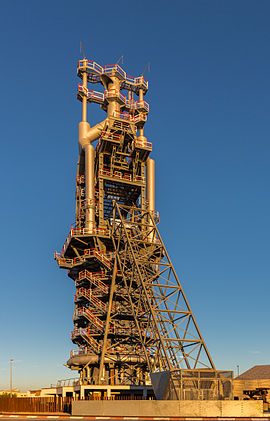
\includegraphics[width=4cm]{altoHorno.jpg}
    \caption{Alto horno.}
  \end{figure}

  Contamos con un modelo matemático, que explicaremos con más detalle en la próxima sección, que nos permite discretizar el dominio del problema y resolverlo por medio de un sistema de ecuaciones lineales. Por lo tanto, serán de interés para nosotros los métodos que permitan encontrar soluciones de este tipo de sistemas de manera computacional.

  Utilizaremos dos métodos diferentes para encarar el problema planteado: el método de Eliminación Gaussiana y el de Factorización LU. Ambos se valen del hecho de que un sistema de ecuaciones puede expresarse en forma matricial, y de que realizando ciertas operaciones sobre las filas de la matriz del sistema, puede obtenerse un sistema equivalente, que tiene las mismas soluciones. Más aún, puede probarse que todo sistema es equivalente a otro cuya matriz es triangular, y encontrar la solución de este tipo de sistemas es sumamente sencillo, utilizando los algoritmos de sustitución hacia adelante o sustitución hacia atrás.

  El método de \emph{Eliminación Gaussiana} itera sobre las columnas de la matriz, colocando ceros en todas las posiciones que se encuentran por debajo de la diagonal. Para hacer esto, en la $i$-ésima iteración, se resta a todas las filas a partir de la $i + 1$ un múltiplo de la fila $i$-ésima, con un factor elegido convenientemente. Esto asegura que, al completar el algoritmo, la matriz obtenida será triangular superior.

  En su forma más básica, el método falla si en alguna iteración se anula el elemento de la diagonal correspondiente a la columna sobre la que se está trabajando. Para salvar esta dificultad, se utiliza una técnica conocida como \emph{pivoteo}, que consiste en alterar el orden de las filas o de las columnas de la matriz. Sin embargo, como probaremos más adelante, la matriz asociada al sistema que estudiaremos tiene la particularidad de que el algoritmo de Eliminación Gaussiana puede aplicarse sin realizar pivoteo.

  El método de \emph{Factorización LU}, por su parte, aprovecha el hecho de que bajo ciertas condiciones, una matriz $A$ puede factorizarse como el producto de otras dos, en la forma $A = LU$, donde $L$ es triangular inferior con unos en la diagonal, y $U$ es triangular superior. De esta manera, el sistema $Ax=b$ puede reescribirse como $LUx=b$, y luego ser resuelto en dos etapas sencillas: si llamamos $y=Ux$, podemos resolver primero el sistema $Ly=b$ (aplicando sustitución hacia adelante, pues $L$ es triangular inferior), y una vez conocido el valor de $y$, resolver $Ux=y$ (aplicando esta vez sustitución hacia atrás), obteniendo así la solución del sistema original.
